% The trivial bundle S^1 x R drawn as an open cylinder.
% Compile with: lualatex -> dvisvgm --pdf.
\documentclass[tikz,border=10pt]{standalone}
\usepackage{amsmath,amssymb}
\usetikzlibrary{arrows.meta}

\definecolor{ink}{HTML}{22303A}
\definecolor{muted}{HTML}{7C8792}
\definecolor{accent}{HTML}{C2410C}
\definecolor{teal}{HTML}{0F766E}
\definecolor{paper}{HTML}{F5ECDD}

\begin{document}
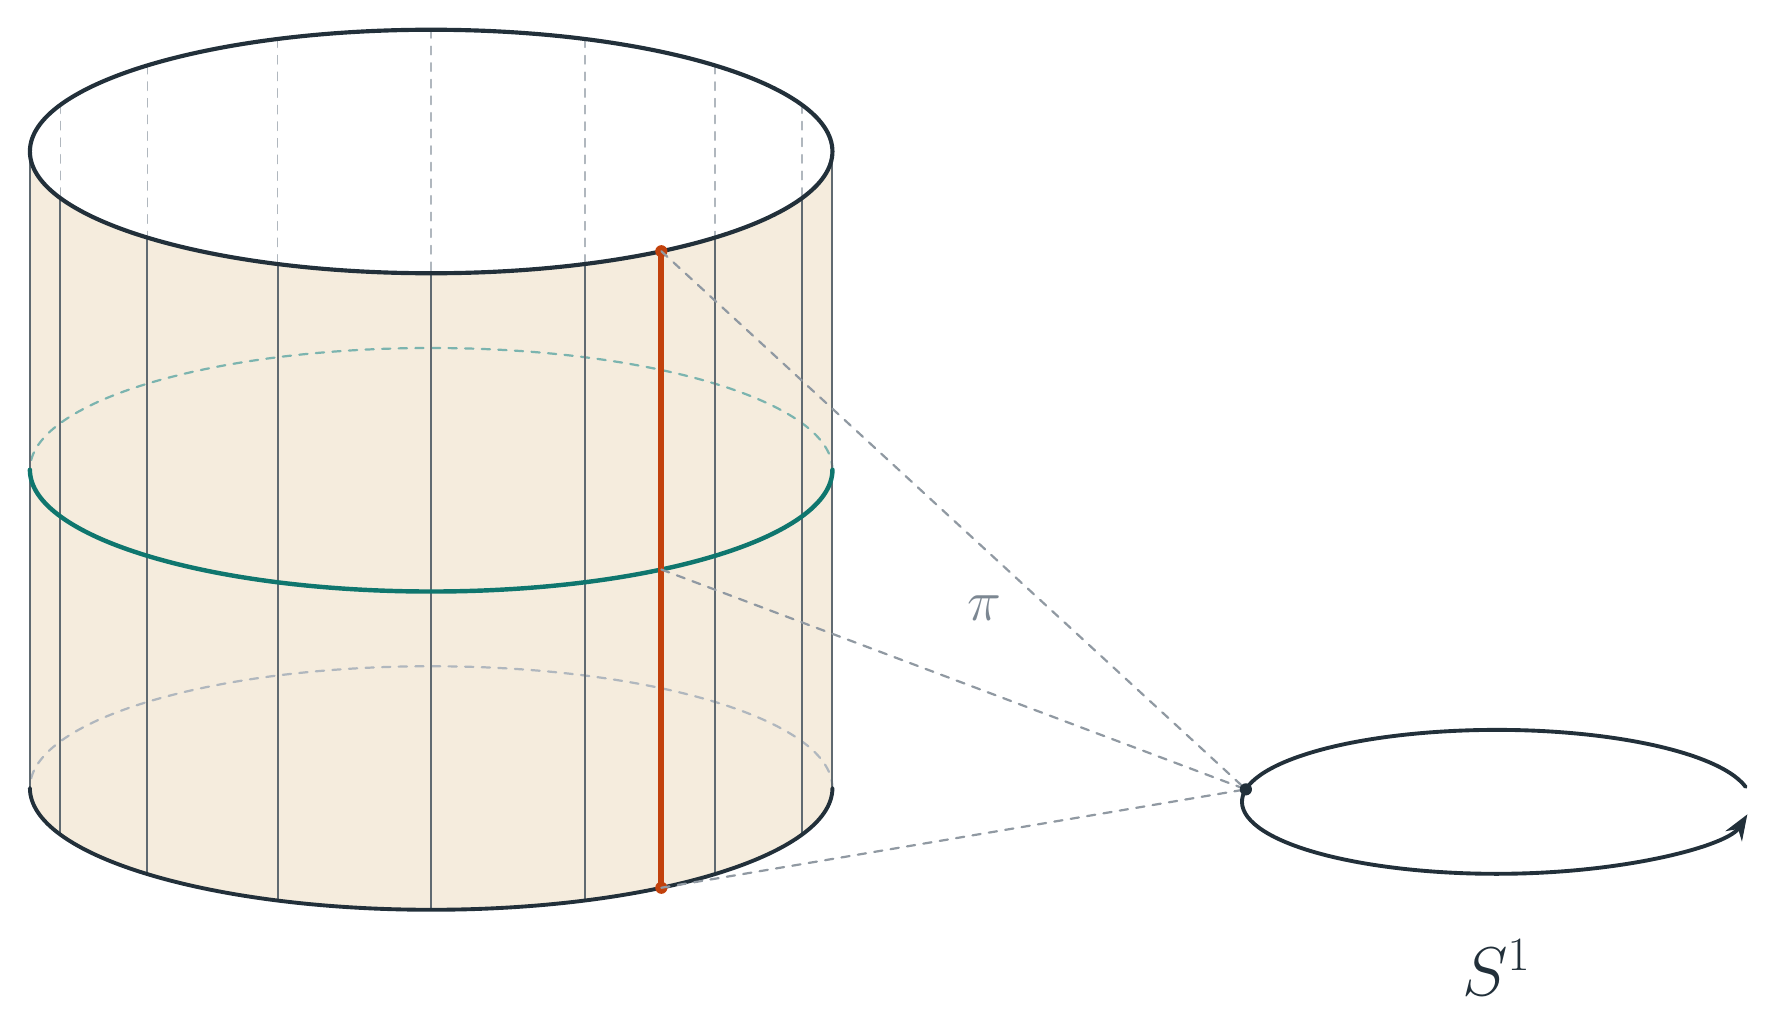
\begin{tikzpicture}[x=1pt,y=1pt,line cap=round,line join=round,>=Stealth]
  % Total space on the left, base circle on the right.
  \def\cx{270}
  \def\R{145}
  \def\ry{44}
  \def\ytop{410}
  \def\ybot{180}
  \def\ymid{295}
  \def\bx{655}
  \def\by{175}
  \def\brx{92}
  \def\bry{26}

  % Body: silhouette with the top opening cut out.
  \fill[paper, even odd rule]
    (\cx-\R,\ytop)
      arc[start angle=180, end angle=0, x radius=\R, y radius=\ry]
      -- (\cx+\R,\ybot)
      arc[start angle=0, end angle=-180, x radius=\R, y radius=\ry]
      -- cycle
    (\cx,\ytop) ellipse[x radius=\R, y radius=\ry];

  % Fibres on the far side (hidden, drawn dashed over the paper).
  \foreach \a in {0,22.5,...,337.5} {
    \pgfmathsetmacro{\x}{\cx+\R*cos(\a)}
    \pgfmathsetmacro{\yt}{\ytop+\ry*sin(\a)}
    \pgfmathsetmacro{\yb}{\ybot+\ry*sin(\a)}
    \pgfmathsetmacro{\front}{sin(\a)<=0.01 ? 1 : 0}
    \ifnum\front=1
    \else
      \draw[muted!60, dashed, line width=0.6pt] (\x,\yt) -- (\x,\yb);
    \fi
  }

  % Far half of the bottom rim and zero section.
  \draw[muted!60, dashed, line width=0.8pt]
    (\cx+\R,\ybot) arc[start angle=0, end angle=180, x radius=\R, y radius=\ry];
  \draw[teal!55, dashed, line width=0.8pt]
    (\cx+\R,\ymid) arc[start angle=0, end angle=180, x radius=\R, y radius=\ry];

  % Near fibres.
  \foreach \a in {0,22.5,...,337.5} {
    \pgfmathsetmacro{\x}{\cx+\R*cos(\a)}
    \pgfmathsetmacro{\yt}{\ytop+\ry*sin(\a)}
    \pgfmathsetmacro{\yb}{\ybot+\ry*sin(\a)}
    \pgfmathsetmacro{\front}{sin(\a)<=0.01 ? 1 : 0}
    \ifnum\front=1
      \draw[ink!72, line width=0.7pt] (\x,\yt) -- (\x,\yb);
    \fi
  }

  % Near half of the bottom rim, then the full top rim.
  \draw[ink, line width=1.4pt]
    (\cx+\R,\ybot) arc[start angle=0, end angle=-180, x radius=\R, y radius=\ry];
  \draw[ink, line width=1.5pt]
    (\cx,\ytop) ellipse[x radius=\R, y radius=\ry];

  % Near half of the zero section.
  \draw[teal, line width=1.6pt]
    (\cx+\R,\ymid) arc[start angle=0, end angle=-180, x radius=\R, y radius=\ry];

  % Highlighted fibre, just right of centre.
  \pgfmathsetmacro{\ah}{-55}
  \pgfmathsetmacro{\xh}{\cx+\R*cos(\ah)}
  \pgfmathsetmacro{\yth}{\ytop+\ry*sin(\ah)}
  \pgfmathsetmacro{\ybh}{\ybot+\ry*sin(\ah)}
  \draw[accent, line width=2.1pt] (\xh,\yth) -- (\xh,\ybh);
  \fill[accent] (\xh,\yth) circle[radius=2.2pt];
  \fill[accent] (\xh,\ybh) circle[radius=2.2pt];

  % Projection fan to the base circle.
  \pgfmathsetmacro{\bah}{170}
  \pgfmathsetmacro{\bpx}{\bx+\brx*cos(\bah)}
  \pgfmathsetmacro{\bpy}{\by+\bry*sin(\bah)}
  \pgfmathsetmacro{\ymidh}{(\yth+\ybh)/2}
  \foreach \y in {\yth,\ymidh,\ybh} {
    \draw[muted!85, dashed, line width=0.8pt] (\xh,\y) -- (\bpx,\bpy);
  }
  \fill[ink] (\bpx,\bpy) circle[radius=2.2pt];

  % Base circle S^1, with a gap and an arrow.
  \draw[ink, line width=1.4pt, -{Stealth}]
    ({\bx+\brx*cos(12)},{\by+\bry*sin(12)})
    arc[start angle=12, end angle=350, x radius=\brx, y radius=\bry];
  \node[ink, font=\fontsize{26}{30}\selectfont] at (\bx,\by-60) {$S^1$};

  % Projection label, in the empty space above the middle ray.
  \node[muted, font=\fontsize{22}{26}\selectfont] at (470,245) {$\pi$};
\end{tikzpicture}
\end{document}
